\documentclass{beamer}
\usetheme{Madrid}
\usepackage{pifont}
\usepackage{amsmath}
\usepackage{geometry} 
\usepackage{svg}
\usepackage{graphicx}
\usepackage{tikz}

\graphicspath{ {./assets/} }
\usetikzlibrary{positioning}



\title{Adaptasi Positional Encoding pada Arsitektur Transformer untuk Sintesis Notasi Gamelan yang Koheren dan Terkendali}
\author{Arif Akbarul Huda}

\begin{document}
	\begin{frame}
		\titlepage
	\end{frame}

	\begin{frame}
		\frametitle{Rumusan Masalah}
		Model LSTM pembangkit notasi gamelan yang dikembangkan oleh Fanani, A.Z. dkk. (2025) gagal menangkap relasi tersirat antarnotasi. Mekanisme pengacakan Algoritma Genetika (GA) digunakan Fanani, A.Z. dkk. (2025) untuk menangani kelemahan LSTM tersebut, tetapi GA justru berpotensi merusak struktur koherensi seluruh notasi. Kondisi tersebut mengakibatkan peran notasi terhadap keseluruhan struktur terabaikan sehingga ciri khas notasi dan identitas musikal gamelan memudar seiring bertambah panjangnya sekuens notasi. Apabila hal ini tidak diatasi, koherensi tematik dalam komposisi notasi gamelan tidak terwujud. Oleh karena itu diperlukan pendekatan baru, model pembangkit notasi gamelan yang dapat mempertimbangkan peran tersirat setiap notasi dalam struktur lagu melalui mekanisme perhatian (attention mechanism).
	\end{frame}
	
	
	\begin{frame}
		\frametitle{Previous Work}
		\framesubtitle{Original vs Rebuild - LSTM}
		\tiny Syarif AM, Azhari A, Suprapto S, Hastuti K. Gamelan Melody Generation Using LSTM Networks Controlled by Composition Meter Rules and Special Notes. JAIT [Internet]. 2023 [cited 2025 June 9]; Available from: http://www.jait.us/show-224-1287-1.html
		% Begin the columns environment
		\begin{columns}
			
			% --- First Column (Left Image) ---
			\begin{column}{0.5\textwidth}
				\begin{figure}
					\centering
					\includegraphics[height=0.75 \linewidth]{original-lstm.png}
					\caption{Original}			
				\end{figure}		
			\end{column}
			
			% --- Second Column (Right Image) ---
			\begin{column}{0.5\textwidth}
				\begin{figure}
					\centering
					\includegraphics[height=0.75 \linewidth]{reverse-code-40hl.png}
					\caption{Rebuild}			
				\end{figure}		
			\end{column}
			
		\end{columns}
		
	\end{frame}
	
	\begin{frame}
		\frametitle{Insight}
		\begin{figure}
			\centering
			\includegraphics[height=0.5 \linewidth]{fisika-bunyi-gamelan.png}
			\caption{Buku Referensi}			
		\end{figure}
	\end{frame}

	\begin{frame}
		\frametitle{Insight}
		\begin{figure}
			\centering
			\includegraphics[width=1 \linewidth]{frekuensi-slendro-pelog.png}
			\caption{Frekuensi fundamental tiap nada gender}			
		\end{figure}
	\end{frame}

	
	
	\begin{frame}
		\frametitle{Insight}
		\begin{figure}
			\centering
			\includegraphics[height=0.5 \linewidth]{interval-in-cent.png}
			\caption{Struktur interval dalam cent antara slendro, pelog dan western}			
		\end{figure}
	\end{frame}

	\begin{frame}
		\frametitle{Insight}
		\begin{figure}
			\centering
			\includegraphics[height=0.5 \linewidth]{bunyi-overtone-harmoni.png}
			\caption{Kempul nada 6}			
		\end{figure}
	\end{frame}

	\begin{frame}
		\frametitle{Insight}
		\framesubtitle{Kenong pada laras slendro}

		% Begin the columns environment
		\begin{columns}
			
			% --- First Column (Left Image) ---
			\begin{column}{0.5\textwidth}	
				\begin{center}
					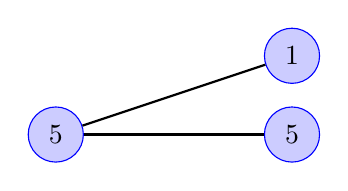
\begin{tikzpicture}[
						% Define a style for all nodes (optional, but helpful)
						node style/.style={circle, draw=blue, fill=blue!20, minimum size=7mm}
						]
						
						% Define and place your nodes
						\node[node style] (A) at (0, 0) {5};
						\node[node style] (B) at (3, 1) {1};
						\node[node style] (C) at (3, 0) {5};
						
						% --- Draw the edges ---
						\draw[thick] (A) -- (B); 
						\draw[thick] (A) -- (C); 
					\end{tikzpicture}
					\vspace{12pt}
					\par %
					{Kenong nada 5 digunakan untuk me-ngenongi nada 1 dan 5}
				\end{center}	
			\end{column}
			
			% --- Second Column (Right Image) ---
			\begin{column}{0.5\textwidth}
				\begin{center}
					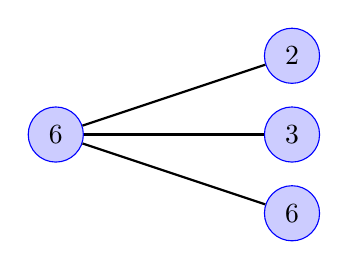
\begin{tikzpicture}[
						% Define a style for all nodes (optional, but helpful)
						node style/.style={circle, draw=blue, fill=blue!20, minimum size=7mm}
						]
						
						% Define and place your nodes
						\node[node style] (A) at (0, 0) {6};
						\node[node style] (B) at (3, 1) {2};
						\node[node style] (C) at (3, 0) {3};
						\node[node style] (D) at (3, -1) {6};
						
						% --- Draw the edges ---
						\draw[thick] (A) -- (B); 
						\draw[thick] (A) -- (C); 
						\draw[thick] (A) -- (D); 
					\end{tikzpicture}
					\vspace{12pt}
					\par %
					{Kenong nada 6 digunakan untuk me-ngenongi nada 2,3 dan 6}
				\end{center}
						
			\end{column}
			
		\end{columns}
		
	\end{frame}


	\begin{frame}
		\frametitle{Insight}
		\framesubtitle{Patet}
		Penggunaan kempyung memiliki relasi dengan patet.
		
		% Begin the columns environment
		\begin{columns}
			
			% --- First Column (Left Image) ---
			\begin{column}{0.5\textwidth}	
				\begin{center}
					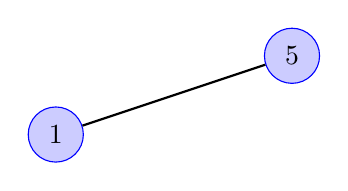
\begin{tikzpicture}[
						% Define a style for all nodes (optional, but helpful)
						node style/.style={circle, draw=blue, fill=blue!20, minimum size=7mm}
						]
						
						% Define and place your nodes
						\node[node style] (A) at (0, 0) {1};
						\node[node style] (B) at (3, 1) {5};
						
						% --- Draw the edges ---
						\draw[thick] (A) -- (B); 
					\end{tikzpicture}
					\par %
					\vspace{12pt}
					\textbf{Patet Sanga}
					\par %
					{Nada seleh 1 diberi kempyung 5}
				\end{center}
			\end{column}
			
			% --- Second Column (Right Image) ---
			\begin{column}{0.5\textwidth}
				\begin{center}
					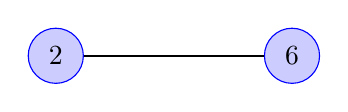
\begin{tikzpicture}[
						% Define a style for all nodes (optional, but helpful)
						node style/.style={circle, draw=blue, fill=blue!20, minimum size=7mm}
						]
						
						% Define and place your nodes
						\node[node style] (A) at (0, 0) {2};
						\node[node style] (B) at (3, 0) {6};
						
						% --- Draw the edges ---
						\draw[thick] (A) -- (B); 
					\end{tikzpicture}
				\par %
				\vspace{12pt}
				\textbf{Patet Nem dan Manyura}
				\par %
				{Nada kenong seleh 2 diberi kempul 6}
				\end{center}
			\end{column}
			
		\end{columns}
		
	\end{frame}


	\begin{frame}
		\frametitle{Experiment}
		\begin{figure}
			\centering
			\includegraphics[height=0.5 \linewidth]{plot-struktur-gamelan.png}
			\caption{Buku Referensi}			
		\end{figure}
	\end{frame}
	

	\begin{frame}
		\frametitle{Experimental Ideas}	% Begin the columns environment
		
		% 1. TOP ROW: TWO COLUMNS (50% each)
		\begin{columns}
			% --- Left Column (Row 1, Col 1) ---
			\begin{column}{0.48\textwidth}
				\centering
				\includegraphics[width=0.9\linewidth]{notasi-ayak-nem-slendro.png}
				\footnotesize{Notasi gamelan Ayak-ayakan Nem Slendro pt. Nem}
			\end{column}
			
			% --- Right Column (Row 1, Col 2) ---
			\begin{column}{0.48\textwidth}
				\centering
				\textbf{Figure B}
				\includegraphics[width=0.9\linewidth]{cmap-font-balungan.png}
				\footnotesize{Cmap font balungan.}
			\end{column}
		\end{columns}
		
		% Optional: Add a small vertical space between the rows
		\vspace{0.5em}
		\hrule % Optional: A horizontal line to visually separate the rows
		
		% 2. BOTTOM ROW: ONE MERGED COLUMN
		% We use \vfill to push the content to the bottom and a minipage to control its width
		\vfill 
		\begin{minipage}{\textwidth} % Minipage spans the full text width
			\centering
			
			\begin{figure}
				\centering
				\includegraphics[width=1 \linewidth]{notasi-ayak-nem-slendro-decoded.png}
				\caption{Notasi ayakan decoded}			
			\end{figure}
		\end{minipage}
		
	\end{frame}

	\begin{frame}
		\frametitle{Experimental Ideas}	% Begin the columns environment
		\begin{columns}
		
			% --- First Column (Left Image) srepeg-tlutur-sl-sanga.png---
			\begin{column}{0.5\textwidth}
				\begin{figure}
					\centering
					\includegraphics[width=1 \linewidth]{srepeg-tlutur-sl-sanga.png}
					\caption{Notasi Gamelan}			
				\end{figure}		
			\end{column}
			
			% --- Second Column (Right Image) ---
			\begin{column}{0.5\textwidth}
				\begin{figure}
					\centering
					\includegraphics[width=1 \linewidth]{plot-struktur-gamelan.png}
					\caption{Plot Struktur}			
				\end{figure}		
			\end{column}
		\end{columns}
	\end{frame}
	
	

	\begin{frame}
			\begin{figure}
			\centering
			\includegraphics[width=0.7\linewidth]{pitch-mismatch.png}
			\caption{Contoh pitch mismatch method}			
		\end{figure}
	
	Fu X, Deng H, Yuan X, Hu J. Generating High Coherence Monophonic Music Using Monte-Carlo Tree Search. IEEE Trans Multimedia. 2023;25:3763–72. 
	\end{frame}

	\begin{frame}
		\frametitle{P.O.C}
		\begin{itemize}
			\item Bagana membuktikan incoherence?
			\item Reverese Paper :  LSTM, BiLSTM, G.A. Small prev dataset Gamelan
			\item Objective : Function untuk scoring tingkat coherence pada gamelan
		\end{itemize}
	\end{frame}
	
\end{document}
